\documentclass{standalone}% For the example only, any class will do
\usepackage{tikz}
\begin{document}

\tikzset{every picture/.style={line width=0.75pt}} %set default line width to 0.75pt

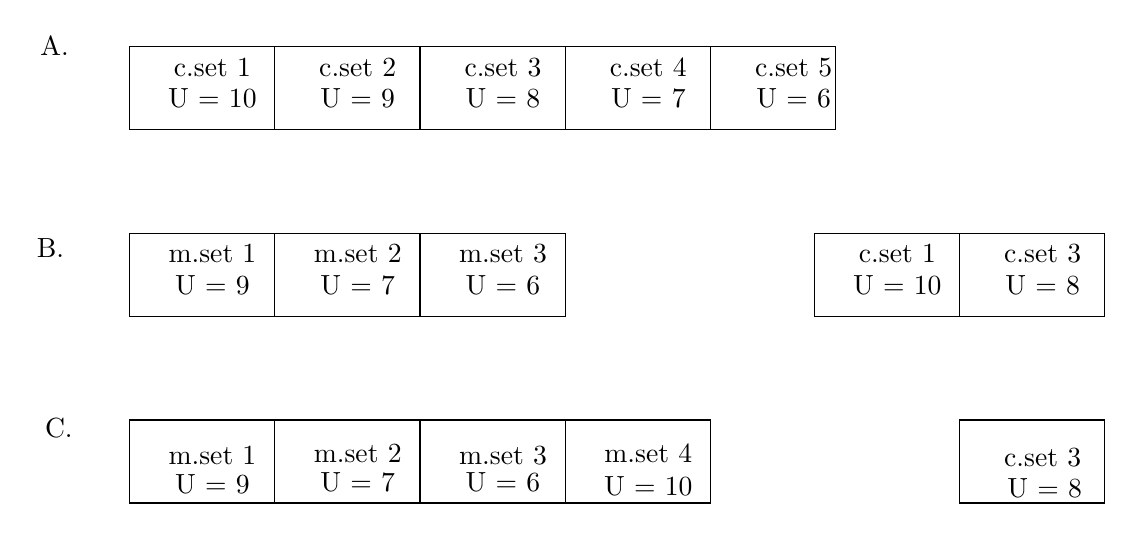
\begin{tikzpicture}[x=0.75pt,y=0.75pt,yscale=-1,xscale=1]
%uncomment if require: \path (0,300); %set diagram left start at 0, and has height of 300

%Shape: Rectangle [id:dp7250426740302982]
\draw   (80,20) -- (150,20) -- (150,60) -- (80,60) -- cycle ;
%Shape: Rectangle [id:dp19598892203956586]
\draw   (150,20) -- (220,20) -- (220,60) -- (150,60) -- cycle ;
%Shape: Rectangle [id:dp914371541975602]
\draw   (220,20) -- (290,20) -- (290,60) -- (220,60) -- cycle ;
%Shape: Rectangle [id:dp7678928301688219]
\draw   (290,20) -- (360,20) -- (360,60) -- (290,60) -- cycle ;
%Shape: Rectangle [id:dp6763737885734915]
\draw   (360,20) -- (420,20) -- (420,60) -- (360,60) -- cycle ;
%Shape: Rectangle [id:dp9387137032109147]
\draw   (410,110) -- (480,110) -- (480,150) -- (410,150) -- cycle ;
%Shape: Rectangle [id:dp37412079551859323]
\draw   (150,110) -- (220,110) -- (220,150) -- (150,150) -- cycle ;
%Shape: Rectangle [id:dp16454361789082173]
\draw   (220,110) -- (290,110) -- (290,150) -- (220,150) -- cycle ;
%Shape: Rectangle [id:dp9175756462958762]
\draw   (80,110) -- (150,110) -- (150,150) -- (80,150) -- cycle ;
%Shape: Rectangle [id:dp15047539733105797]
\draw   (480,110) -- (550,110) -- (550,150) -- (480,150) -- cycle ;
%Shape: Rectangle [id:dp26374479334036427]
\draw   (80,240) -- (150,240) -- (150,200) -- (80,200) -- cycle ;
%Shape: Rectangle [id:dp6792148953471306]
\draw   (150,200) -- (220,200) -- (220,240) -- (150,240) -- cycle ;
%Shape: Rectangle [id:dp363147733856537]
\draw   (220,200) -- (290,200) -- (290,240) -- (220,240) -- cycle ;
%Shape: Rectangle [id:dp5611568263873337]
\draw   (290,200) -- (360,200) -- (360,240) -- (290,240) -- cycle ;
%Shape: Rectangle [id:dp23010587717062214]
\draw   (480,200) -- (550,200) -- (550,240) -- (480,240) -- cycle ;

% Text Node
\draw (120,30) node  [align=left] {c.set 1};
% Text Node
\draw (190,30) node  [align=left] {c.set 2};
% Text Node
\draw (260,30) node  [align=left] {c.set 3};
% Text Node
\draw (330,30) node  [align=left] {c.set 4};
% Text Node
\draw (400,30) node  [align=left] {c.set 5};
% Text Node
\draw (120,120) node  [align=left] {m.set 1};
% Text Node
\draw (190,120) node  [align=left] {m.set 2};
% Text Node
\draw (450,120) node  [align=left] {c.set 1};
% Text Node
\draw (260,120) node  [align=left] {m.set 3};
% Text Node
\draw (520,120) node  [align=left] {c.set 3};
% Text Node
\draw (120,217) node  [align=left] {m.set 1};
% Text Node
\draw (190,216) node  [align=left] {m.set 2};
% Text Node
\draw (260,217) node  [align=left] {m.set 3};
% Text Node
\draw (330,216) node  [align=left] {m.set 4};
% Text Node
\draw (520,218) node  [align=left] {c.set 3};
% Text Node
\draw (120,45) node  [align=left] {U = 10};
% Text Node
\draw (190,45) node  [align=left] {U = 9};
% Text Node
\draw (260,45) node  [align=left] {U = 8};
% Text Node
\draw (330,45) node  [align=left] {U = 7};
% Text Node
\draw (400,45) node  [align=left] {U = 6};
% Text Node
\draw (120,135) node  [align=left] {U = 9};
% Text Node
\draw (190,135) node  [align=left] {U = 7};
% Text Node
\draw (260,135) node  [align=left] {U = 6};
% Text Node
\draw (450,135) node  [align=left] {U = 10};
% Text Node
\draw (520,135) node  [align=left] {U = 8};
% Text Node
\draw (120,231) node  [align=left] {U = 9};
% Text Node
\draw (190,230) node  [align=left] {U = 7};
% Text Node
\draw (260,230) node  [align=left] {U = 6};
% Text Node
\draw (330,232) node  [align=left] {U = 10};
% Text Node
\draw (521,233) node  [align=left] {U = 8};
% Text Node
\draw (44,20) node  [align=left] {A.};
% Text Node
\draw (42,117) node  [align=left] {B.};
% Text Node
\draw (46,204) node  [align=left] {C.};
\end{tikzpicture}


\end{document}
